% !TeX root = ../thuthesis-example.tex

\chapter{PROTOTYPE OF VR-IoT Research Platform}

\section{Platform requirements}
Firstly, we define the requirements our platform should follow:
\begin{enumerate}
\item Scalability. The performance of the platform should stay acceptable when the number of devices in our system increase;
\item Ease of use and testing. Since using Virtual Reality and IoT devices requires interacting with different kinds of elements, we need to provide a natural way of interacting with such objects. As for real-world devices we only need to implement sensor data collection, creating an API for virtual reality digital representation of such devices can be a challenge. Another important task is simulation of VR interactions on a computer for ease of testing;
\item Fault Tolerance. As if we are not developing the IoT devices themselves, platform should effectively handle faults coming from both sides (real and virtual worlds);
\item Simultaneous work. As in the real world, when several people can interact with an IoT system, each of the running instances of the platform should be able to run simultaneously and operate with the same data.
\end{enumerate}
The architecture of the platform has to be based on three layers, which we further modify and extend with extra connections: 
\begin{enumerate}
    \item Real-world IoT devices HUB. In order to collect the data from real-world devices, we need a special device responsible for receiving and sending the data to them. In commercial market, usually mobile phone apps have interface to interact with IoT devices (Mi Home APP, HomeKit App etc), but since we require using the data in virtual reality (which is a different interface), we need to operate with IoT sensors data on a special HUB, which can provide the data in a unified format (abstraction of sensors)
    \item Integration layer. This is the main part of the platform. Analyzing data coming from VR and from real world, integrating real-world devices data into VR and vice-versa, performing persistence and providing API for using the platform in research projects;
    \item Visualization layer. Interaction with digital IoT devices can be performed using VR headsets, AR devices or by simulating the touch, sight, gestures and other interactions. Our aim is to provide an API for developers to integrate their interaction techniques into this layer, but developing these techniques is not the focus of this research. 
\end{enumerate}

\section{Real-world IoT devices HUB}
To support different IoT devices in out platform, either a standalone or third-party software can be used. By analyzing the market, we have agreed on using a third-party software openHAB with a future upgrade to our own solution. The Hub we use runs on a server and is responsible for collecting and storing the data coming from IoT devices. Managing the data is performed through a web interface, while API is based on REST calls.

\section{Integration layer}
By receiving and sending unified data objects representing IoT devices sensor data using REST API calls, each of the running instances of the NUIX-Studio App (our platform) running in the Integration layer will operate with the same data, enabling simultaneous work.
Next step is to represent IoT devices data in virtual reality and perform computations for research. Since the platform should run smoothly on VR headsets and provide good UX, the computations should be performed on a high-performance PC, while interaction with virtual IoT devices is done by using VR headsets. 

\section{Visualization layer}
Since the platform purpose is to provide an API for research on IoT devices in VR, we decided to use Unity for interaction with virtual reality devices. First of all, by choosing Unity, we save time from developing our own 3D engine. Secondly, we can build the project for most of platforms and provide support for VR headsets. And thirdly, developers are already familiar with Unity development, and can integrate their research projects into the platform faster than if we used our own 3D engine.

\begin{figure}
  \centering
  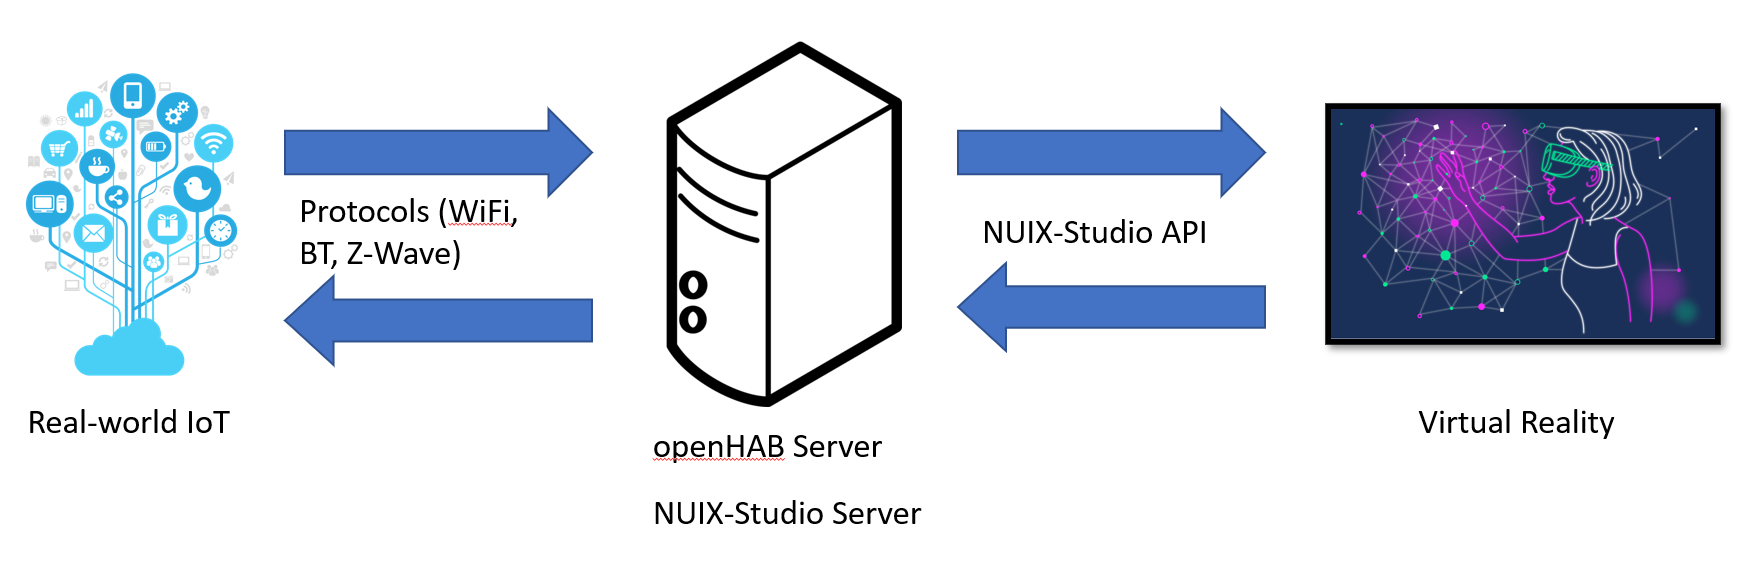
\includegraphics[width=0.6\linewidth]{figures/BasicPlatformStructure.png}
  \caption{Simplified structure of NUIX Studio. Real-world IoT devices HUB is openHAB server, while NUIX-Studio server is the main instance of NUIX-Studio APP responsible for the computations.}
  \label{fig:BasicPlatformStructure-figure}
\end{figure}

\section{Server Architecture}
\subsection{OpenHAB Server Structure}

Before we explain the structure of our server, we first give definitions for the base elements of openHAB:

Things are entities that can be physically added to a system. Things may provide more than one function (for example, a Z-Wave multi-sensor may provide a motion detector and also measure room temperature). Things do not have to be physical devices; they can also represent a web service or any other manageable source of information and functionality.

Things expose their capabilities through Channels. Whether an installation takes advantage of a particular capability reflected by a Channel depends on whether it has been configured to do so. When you configure your system, you do not necessarily have to use every capability offered by a Thing. You can find out what Channels are available for a Thing by looking at the documentation of the Thing's Binding.

Bindings can be thought of as software adapters, making Things available to your home automation system. They are add-ons that provide a way to link Items to physical devices. They also abstract away the specific communications requirements of that device so that it may be treated more generically by the framework.

Items represent capabilities that can be used by applications, either in user interfaces or in automation logic. Items have a State and they may receive commands.

The glue between Things and Items are Links. A Link is an association between exactly one Channel and one Item. If a Channel is linked to an Item, it is "enabled", which means that the capability the Item represents is accessible through that Channel. Channels may be linked to multiple Items and Items may be linked to multiple Channels.

\begin{figure}
  \centering
  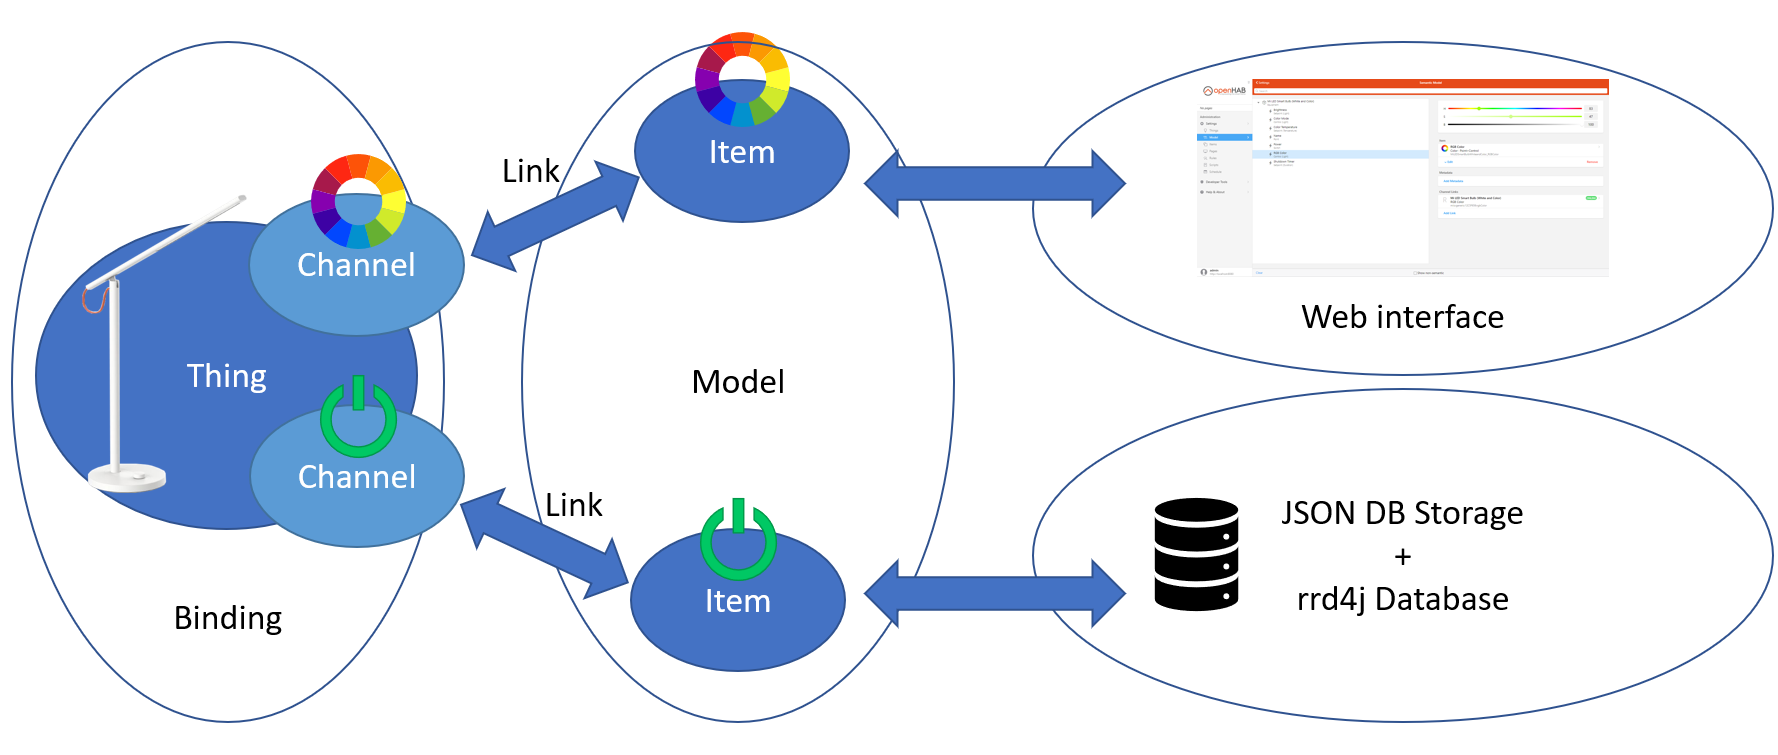
\includegraphics[width=0.9\linewidth]{figures/openHABServerStructure.png}
  \caption{Simplified structure of NUIX Studio. Real-world IoT devices HUB is openHAB server, while NUIX-Studio server is the main instance of NUIX-Studio APP responsible for the computations.}
  \label{fig:openHABServerStructure-figure}
\end{figure}

Overall, the structure may seem a bit difficult for understanding, and that’s why we will focus on only the basic parts in this document:
In our example each of the items is linked only to one channel, and each of the channels is linked to only one item. 

Assume that we installed a binding for Xiaomi smart home devices. The smart home devices we can access have been automatically discovered by our server and added as Things. In our example we are using Xiaomi Lamp, for which several Channels are presented:

Each of these channels represents one item. 

For example, the Power Control is performed through power channel. The power control, in terms of the concepts we introduced, is an item with name MiLEDSmartBulbWhiteandColorPower of type Switch and State “OFF”.

As soon as we turn on the lamp, the power control switch in Web Interface will also turn ON. And if we put the switch to the “OFF” state in the Web Interface, the lamp will turn off.

To support Fault Tolerance, our openHAB server stores data over time.

\subsection{Server Extended Structure}

In the previous paragraph we didn’t specify how our platform should perform access to the server data. 

\begin{figure}
  \centering
  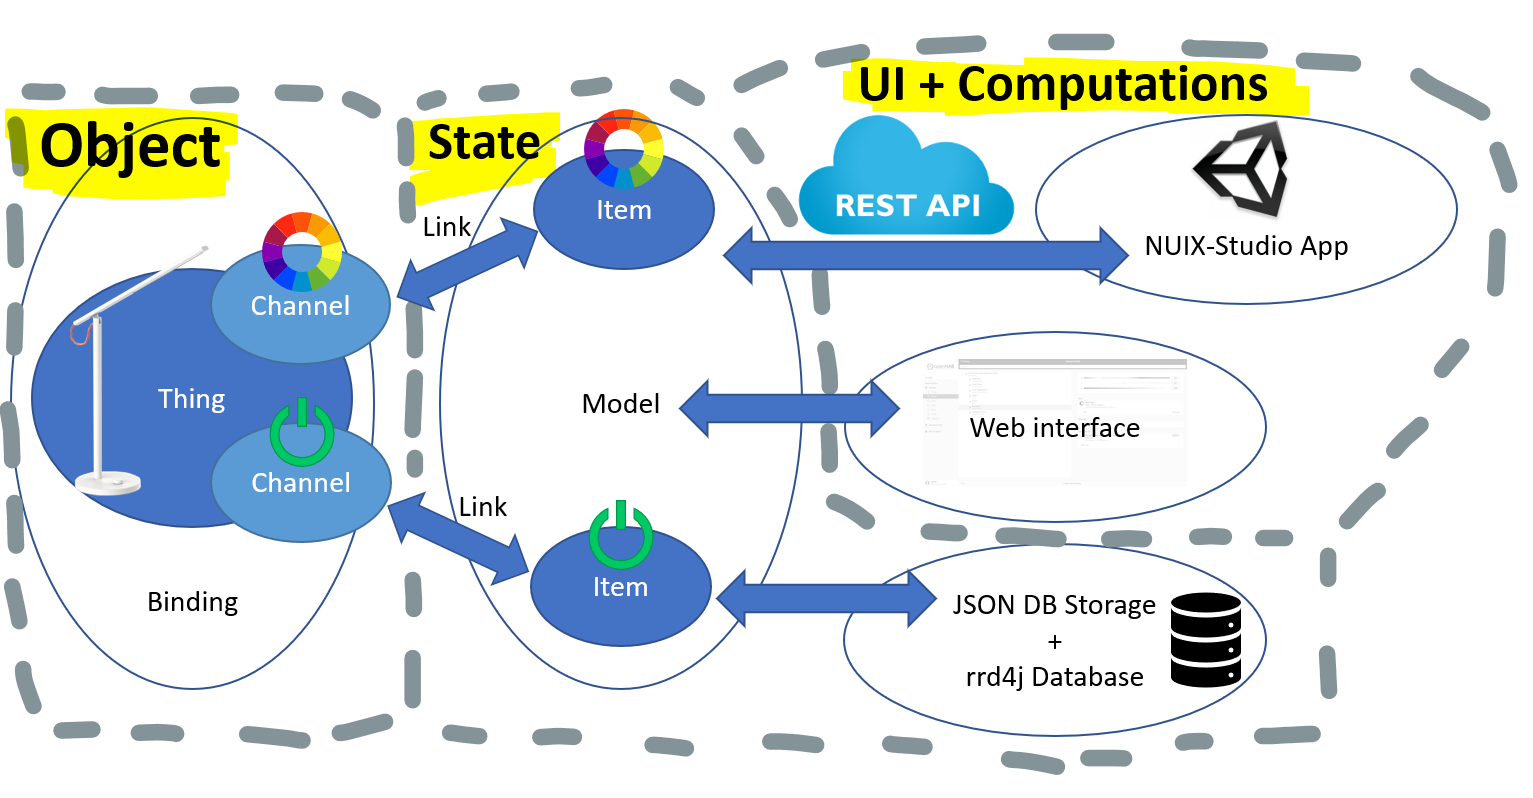
\includegraphics[width=0.9\linewidth]{figures/ExtendedServerStructure.png}
  \caption{Structure of the server showing how the NUIX-Studio APP is connected to it.}
  \label{fig:ExtendedServerStructure-figure}
\end{figure}

As seen in Table~\ref{tab:three-part-table}, syncing is performed through REST API, which is explained in details further.

\begin{table}
  \centering
  \begin{threeparttable}[c]
    \caption{REST API commands used in NUIX-Studio}
    \label{tab:three-part-table}
    \begin{tabular}{ll}
      \toprule
      REST API CALL    &         DESCRIPTION                 \\
      \midrule
      GET\tnote{a} & Get all available items \\
      POST\tnote{b} & Adds a new item to the registry or updates the existing item    \\
      PUT\tnote{b}        & Sends a command to the item                              \\
      DELETE\tnote{b}        & Removes an item from the registry          \\
      \bottomrule
    \end{tabular}
    \begin{tablenotes}
      \item [a] For link: /items
      \item [b] For link: /items/<itemname>
    \end{tablenotes}
  \end{threeparttable}
\end{table}

In the current implementation of the platform, 4 different REST API commands are used: GET command for receiving the items in the registry on system startup, PUT command to create a new item on the server, POST command for updating the state of the item, and DELETE command for removing an item from the server.

Receiving the states of the items from the server is performed through getting the events from the server: once the event is received, the item state can be retrieved from payload.

\section{NUIX-Studio APP}

As mentioned above, there can be several NUIX-Studio APP instances running at the same time. Each of them has access and performs syncing to the Server through REST API. The instances can be of one of three types:

\begin{enumerate}
    \item Virtual Reality Instance. Runs on Oculus or another VR headset, has remote or local access to the server. Items received from the server are visualized and it is possible to interact with them using different techniques such as touching buttons, moving sliders, performing gestures using hand recognition, using voice commands etc. 
    \item Computations Instance. Runs on a powerful machine and has either remote or local access to the server. Since latency is important for our platform, it is more preferable to run this instance on the same machine as openHAB. In this case the REST API calls time will be less than minimum measurement unit (compared to milliseconds for accessing remote virtual reality instances). Physics, big data analysis and other performance-based computations are performed on this instance, while interactions are limited.
    \item Input simulation instance. If the APP instance is running on the device with limited support of interaction interfaces (for example, a PC), input simulation can be used. Sometimes, it is even easier to run and test the platform on such devices: for example, if using a physical keyboard is needed, or when there is no access for VR headset at the moment.
\end{enumerate}

\begin{figure}
  \centering
  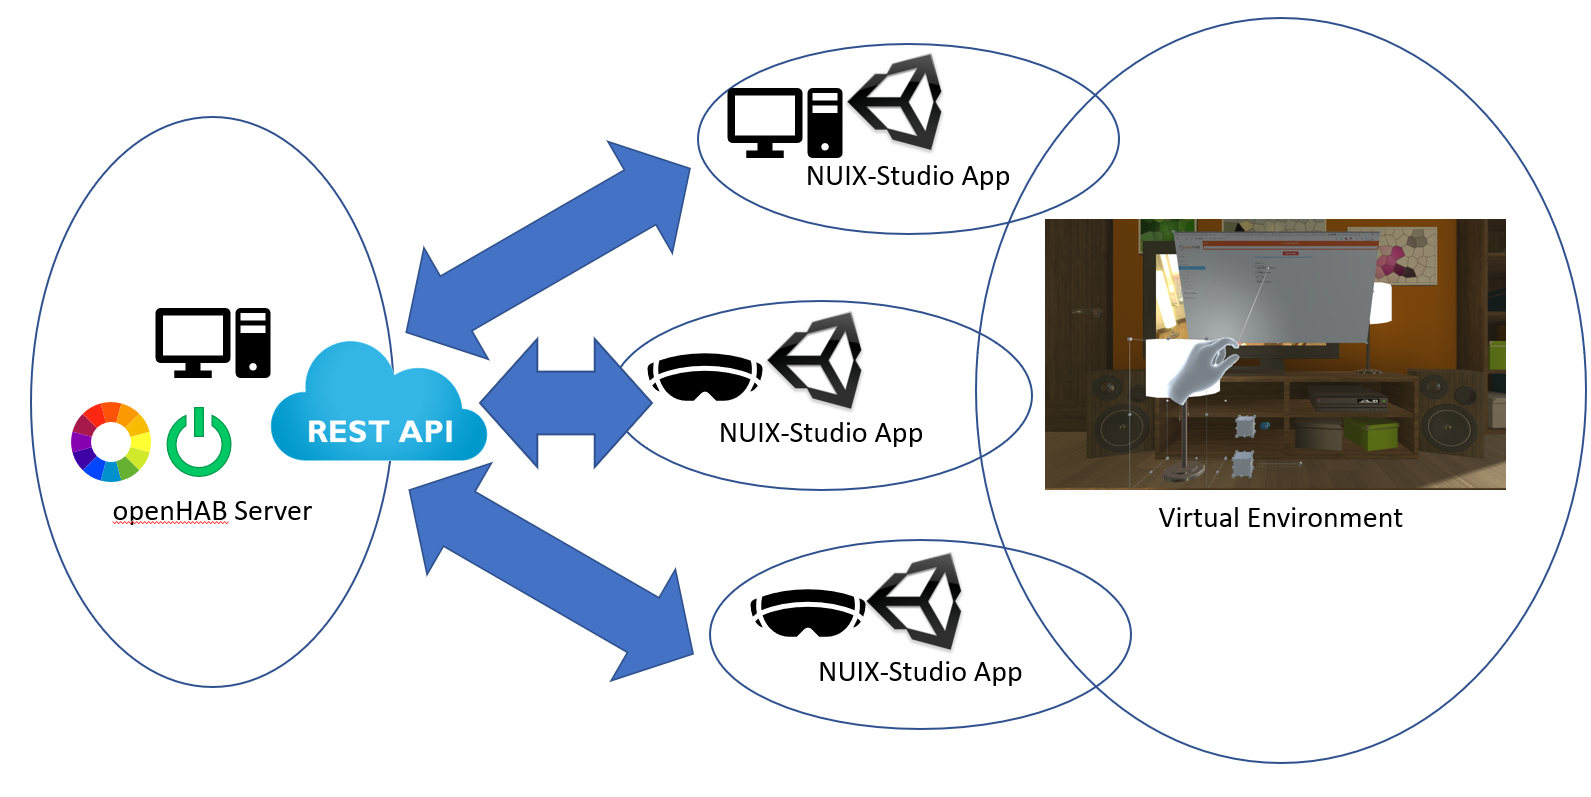
\includegraphics[width=0.9\linewidth]{figures/AppInstances.png}
  \caption{NUIX-Studio App Instances}
  \label{fig:AppInstances-figure}
\end{figure}

Each of the instances performs access to the same data on the server, which makes it possible to work simultaneously in one virtual environment, as well as divide tasks between different instances: as mentioned above, one of the instances can be used for computations, while the other instances for interacting with the devices in virtual reality.

\subsection{NUIX-Studio App Architecture}

When the NUIX-Studio APP requests the access to the system to get the list of items from the registry, a list of Item Data Transfer Objects is received by the app and then added into Semantic Model. When the state of the item is updated, or if a new item is added or removed, an event is sent to the EventController instance, and then, based on the event payload, the item list in updated.  By keeping each item’s data equal to the server, the semantic model in NUIX-Studio APP is equivalent to the semantic model presented on the server. 

But only keeping the states of the items in the APP does not allow us to interact with the items. In other words, NUIX-Studio App has to provide an interface to interact with the items. Since different types of items require different interaction techniques, for each item type a widget is created.
Widget in NUIX-Studio APP is a Unity Virtual GameObject, which can visualize the item state and update it. For example, it can be an interactable pinch slider for a dimmer item, or a virtual screen  for an image item.

By integrating Extra packages, NUIX-Studio platform can provide a bigger variety of widgets, as well as higher number of supported devices. For example, Oculus Integration support provides an API for hands recognition, while Steam VR support makes it possible to run the NUIX-Studio APP on the majority of VR headsets.

\begin{figure}
  \centering
  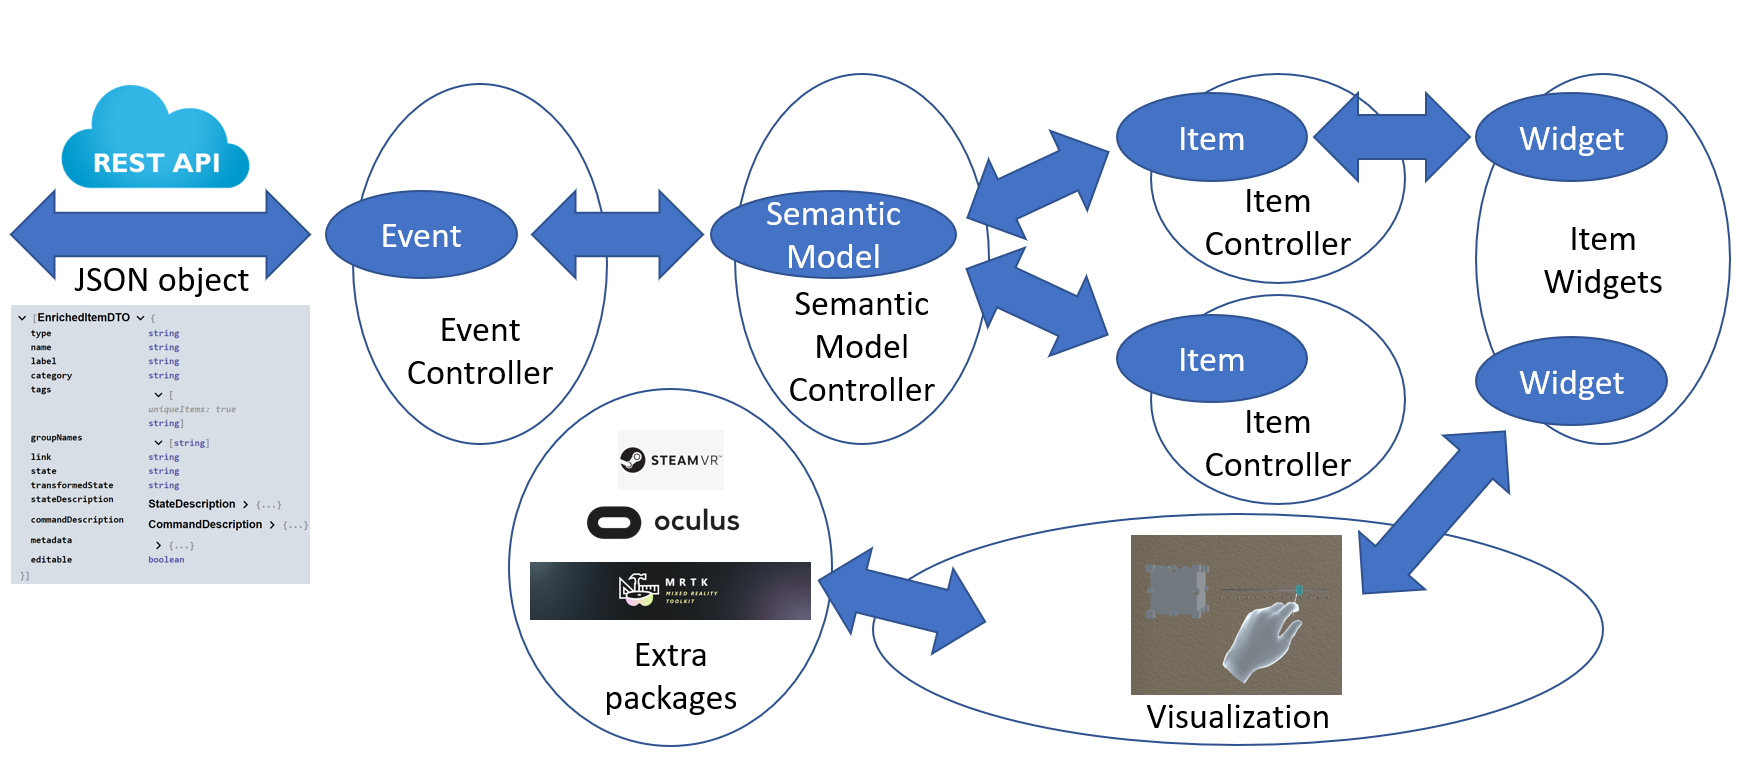
\includegraphics[width=0.9\linewidth]{figures/AppArchitecture.png}
  \caption{NUIX-Studio App Architecture}
  \label{fig:AppArchitecture-figure}
\end{figure}

\subsection{NUIX-Studio APP Semantic Model}

As mentioned above, the semantic model in the NUIX-Studio App is kept equivalent to the semantic model stored on the server. The advantages of this approach are:

\begin{enumerate}
    \item Each of the APP instances visualizes equivalent data, which leads to support of simultaneous and fault-tolerance work;
    \item The semantic model on the server is time and memory effective, and it is better to develop the platform based on such model;
    \item It is more effective solution for using third-party frameworks. Since openHAB is a flexible popular open-source software for IoT systems, in the future, if more functionality is going to used with openHAB, our solution will still be working.
\end{enumerate}

Overall, by using the defined approach, the platform follows Dependency-inversion principle "depend upon abstractions, [not] concretions." In this case, Semantic Model is an abstraction, and Item representation is an abstraction as well.

But in our case, when it is required to provide an interface for creating new IoT devices in VR and interact with them, it is not possible to use only items presented on the server. For example, the virtual position in the environment for each item is an important data, which should be accessible by each of the instances.

Therefore, the disadvantages of keeping the equivalent semantic models are:

\begin{enumerate}
    \item The semantic model should be extended with extra items, such as virtual position or environment setup. These items are needed by each running instance of NUIX-Studio APP.
    \item The main purpose of the platform is to provide an interface to test new IoT devices inside virtual reality, or extend the existing items with extra functionality. But only real-world devices data is stored on the server, therefore it should be extended with virtual items data.
\end{enumerate}

In result, extending the semantic model with virtual items helps us to minimize the number of disadvantages while keeping the advantages.
In the next chapter an example of using the NUIX-Studio is given and the measured performance is analyzed.

\section{Symbols}

As required by the national formatting standards, the template uses \pkg{unicode-math} for formatting mathematical symbols, which differs to the default used by LATEX. 

\begin{enumerate}
  \item Capital Greek letters are italic by default e.g. \cs{Delta}:$\Delta$。
  \item Increment symbol: $\increment$(U+2206)
  \item Vectors, matrices, tensors should be ITALIC, and BOLD using the \cs{symbf} command; for example: $\symbf{A}$, $\symbf{\alpha}$.
  \item For constants and special functions, use the \cs{symup} command. For example:
    $\symup{\pi} = 3.14\dots$; $\symup{e} = 2.718\dots$,
  \item Example of integrals and differentials: $\int f(x) \dif x$。
\end{enumerate}

For more usage of symbols, you could use the following references
\href{http://mirrors.ctan.org/macros/latex/contrib/unicode-math/unicode-math.pdf}{\pkg{unicode-math}}
\href{http://mirrors.ctan.org/macros/latex/contrib/unicode-math/unimath-symbols.pdf}{\pkg{unimath-symbols}}.

For units and metrics, it is recommended to use the following package:
\href{http://mirrors.ctan.org/macros/latex/contrib/siunitx/siunitx.pdf}{\pkg{siunitx}}
It can conveniently handle the space between Greek letters/numbers and the unit. For example:
\SI{6.4e6}{m},
\SI{9}{\micro\meter},
\si{kg.m.s^{-1}},
\SIrange{10}{20}{\degreeCelsius}。



\section{Mathematical formula}

You can use the following environments \env{equation} 和 \env{equation*} for mathematical formulae.

Please pay attention that round brackets should be included before and after referencing an equation: e.g. Equation \eqref{eq:example}.

\begin{equation}
  \frac{1}{2 \symup{\pi} \symup{i}} \int_\gamma f = \sum_{k=1}^m n(\gamma; a_k) \mathscr{R}(f; a_k)
  \label{eq:example}
\end{equation}

When there are multiple equations, please try to align them at the "equal" sign if possible. We recommend using the \env{align} environment.
For example:
\begin{align}
  a & = b + c + d + e \\
    & = f + g
\end{align}


\section{Mathematical axioms and proofs}

You can use \pkg{amsthm} or \pkg{ntheorem} packages to set up your axiom. After loading one of those package, the template will automatically setup the environments: \env{theorem} and \env{proof}

An example:
\begin{theorem}[Lindeberg--Lévy Central Limit Theorem]
  Set random variables $X_1, X_2, \dots, X_n$ i.i.d., with expectation mean of $\mu$ and variance $\sigma^2 \ne 0$. By formula, $\bar{X}_n = \frac{1}{n} \sum_{i+1}^n X_i$, we have
  \begin{equation}
    \lim_{n \to \infty} P \left(\frac{\sqrt{n} \left( \bar{X}_n - \mu \right)}{\sigma} \le z \right) = \Phi(z),
  \end{equation}
  where $\Phi(z)$ is the function of a normal distribution.
\end{theorem}
\begin{proof}
  Trivial.
\end{proof}

The template also provides the following environments: \env{assumption}、\env{definition}、\env{proposition}、
\env{lemma}、\env{theorem}、\env{axiom}、\env{corollary}、\env{exercise}、
\env{example}、\env{remar}、\env{problem}、\env{conjecture} 